\documentclass[../thesis.tex]{subfiles}

\begin{document}

Η εφαρμογή κινητού δημιουργήθηκε χρησιμοποιώντας το framework του Flutter.
Το Flutter επιλέχθηκε ως framework κυρίως λόγω της δυνατότητας που προσφέρει για εύκολη και γρήγορη ανάπτυξη εφαρμογών, και λόγω της απαίτησής μας για cross-platform λειτουργία.
Η ανάπτυξη της εφαρμογής στη native γλώσσα κάθε πλατφόρμας θα απαιτούσε σημαντικά περισσότερο χρόνο, καθώς θα χρειαζόταν να δημιουργήσουμε δύο ανεξάρτητες εφαρμογές (μία για την πλατφόρμα Android, και μία για την πλατφόρμα iOS) γράφοντας πρακτικά τη διπλάσια ποσότητα κώδικα σε δύο διαφορετικές γλώσσες.
Εκτός από τον διπλασιασμό του χρόνου συγγραφής του κώδικα, η ύπαρξη δύο codebase αυξάνει τον αριθμό των ενδεχόμενων σφαλμάτων που μπορεί να προκύψουν, καθιστά σε βάθος χρόνου πιο δύσκολη τη συντήρηση, και απαιτεί επιπλέον προσοχή για τη διασφάλιση της ισότητας των δύο εκδόσεων της εφαρμογής (feature parity).
Αξιοποιώντας το Flutter γράψαμε έναν ενιαίο κώδικα ο οποίος λειτουργεί αμέσως και στις δύο πλατφόρμες, ενώ είμαστε σίγουροι ότι η συμπεριφορά της εφαρμογής θα είναι ίδια για όλους τους χρήστες ανεξαρτήτως της συσκευής που χρησιμοποιούν.

Ως οδηγός, ο χρήστης έχει τη δυνατότητα να προσθέσει στο προφίλ του τα οχήματα που χρησιμοποιεί, προσδιορίζοντας τα χαρακτηριστικά που επιτρέπουν την αναγνώρισή τους από τους πεζούς.
Συγκεκριμένα, για το κάθε όχημα ο χρήστης προσδιορίζει το μοντέλο (επιλέγοντας από μία περιεκτική λίστα) και τον αριθμό πινακίδας.
Προκειμένου να διευκολυνθεί η άμεση αναγνώριση του οχήματος από τους επιβάτες ο χρήστης μπορεί προαιρετικά να προσθέσει το χρώμα αλλά και μία φωτογραφία του.

Πέρα των στοιχείων του οχήματος, ο κάθε χρήστης (πεζός ή οδηγός) μπορεί επίσης προαιρετικά να ανεβάσει μία φωτογραφία προφίλ με την οποία θα παρουσιάζεται στους υπόλοιπους χρήστες.
Τέλος, ο χρήστης έχει μία βαθμολογία η οποία βασίζεται σε όλες τις προηγούμενες αλληλεπιδράσεις τους με άλλους χρήστες της εφαρμογής, αναπαριστώντας την ποιότητα του ως οδηγός ή επιβάτης.

Κατά την έναρξη της εφαρμογής, ο χρήστης παραπέμπεται στην υπηρεσία ταυτοποίησης της σχολής προκειμένου να επαληθευτεί η ταυτότητά του ως φοιτητής.
Κατά την επιτυχή ταυτοποίηση η εφαρμογή ανοίγει μία σύνδεση WebSocket με τον server, στέλνοντας ταυτόχρονα το ΑΜ και το όνομα του φοιτητή.
Σημαντικό είναι το γεγονός ότι η σύνδεση με τον server επιτυγχάνεται μόνο εφόσον έχει επαληθευτεί η ταυτότητα του χρήστη.
Με αυτόν τον τρόπο όχι μόνο απαγορεύεται η χρήση της εφαρμογής από τρίτους, αλλά και ο server προστατεύεται από κακόβουλες ενέργειες.
Ακόμα και αν κάποιος χρήστης επιχειρήσει να κάνει κατάχρηση της εφαρμογής ή να "επιτεθεί" στον server θα πρέπει να έχει ήδη συνδεθεί με τα προσωπικά του στοιχεία, στην οποία περίπτωση η ταυτότητά του μπορεί να προσδιοριστεί και να ληφθούν τα απαραίτητα μέτρα όπως ο αποκλεισμός του συγκεκριμένου λογαριασμού.

Για την ταυτοποίηση χρησιμοποιούμε το AppAuth, έναν OAuth/OpenID Connect client ο οποίος είναι σχεδιασμένος για την επαλήθευση ταυτότητας χρηστών μέσω κινητών εφαρμογών.
Η ταυτοποίηση πραγματοποιείται με ασφαλή τρόπο στη συσκευή και το αποτέλεσμα της είναι ένα token (JWT) που περιέχει τα προσωπικά στοιχεία του χρήστη μαζί με μία "υπογραφή" που πιστοποιεί την αυθεντικότητά του.
Το token αυτό στέλνεται στον server κατά την έναρξη της συνεδρίας πάντα μέσω HTTPS σύνδεσης, και εφόσον επαληθευτεί ως έγκυρο ο server γνωρίζει πια την ταυτότητα του χρήστη πίσω από τη συγκεκριμένη σύνδεση.
Η διαδικασία γίνεται με τέτοιο τρόπο ώστε σε καμία περίπτωση να μη φανερώνεται ο κωδικός λογαριασμού του χρήστη στην εφαρμογή, ενώ η πιθανότητα κλοπής της ταυτότητάς του είναι κατεσταλμένη.
Τα προσωπικά δεδομένα του χρήστη προστατεύονται περαιτέρω καθώς μόνο τα απολύτως απαραίτητα στοιχεία αιτούνται από την εφαρμογή (ΑΜ και όνομα), ο χρήστης πληροφορείται ρητά για την κοινοποίηση των δεδομένων αυτών, και απαιτείται η τελική συναίνεση του για την αποστολή τους στον server.

Μετά από την επιτυχή ταυτοποίηση του, ο χρήστης έχει τη δυνατότητα να επιλέξει το ρόλο του ως οδηγός ή ως επιβάτης.

Η διαδικασία ξεκινάει όταν ο οδηγός πατήσει το κουμπί εκκίνησης, έχοντας προηγουμένως έχει προσδιορίσει το όχημα με το οποίο μετακινείται.
Η εφαρμογή αρχικά παραμένει ανενεργή, παρατηρώντας μόνο το στίγμα του οδηγού έως ότου αυτός πλησιάσει αρκετά στη στάση όπου περιμένουν οι πεζοί.
Σε αυτό το σημείο η εφαρμογή επικοινωνεί με τον server, ρωτώντας για την ύπαρξη πεζών στη στάση, και αν υπάρχουν όντως πεζοί ειδοποιεί τον οδηγό.
Αν ο οδηγός αποδεχτεί, τότε κάποιος από τους πεζούς ορίζεται ως ο επιβάτης του.

Όσον αφορά τον πεζό, η εφαρμογή επίσης παραμένει αρχικά ανενεργή μέχρι κάποιος οδηγός να γίνει διαθέσιμος.
Τότε ένας μικρός αριθμός από πεζούς (το πολύ 5) ειδοποιείται για την ύπαρξη του οδηγού, και ο πρώτος από αυτούς που αποδεχτεί την πρόσκληση ορίζεται ως ο επιβάτης του οδηγού.

Από αυτό το σημείο και πέρα, οδηγός και επιβάτης παρουσιάζονται με τα στοιχεία του αλλουνού (όνομα, αριθμός πινακίδας, φωτογραφίες κτλ.) καθώς και με έναν χάρτη της περιοχής πάνω στον οποίο βρίσκονται τα στίγματά τους.
Ο οδηγός κατευθύνεται προς τον πεζό, και ο πεζός παρατηρεί στον χάρτη τη διαδρομή του οδηγού του.
Μόλις ο οδηγός πλησιάσει στη στάση, και οι δύο τους ειδοποιούνται από την εφαρμογή ώστε ο πεζός να επιβιβαστεί στο όχημα.
Σε περίπτωση που ο οδηγός αποχωρήσει μην έχοντας λάβει τον πεζό, η συνεδρία τους ακυρώνεται και η εφαρμογή του πεζού συνεχίζει να αναζητά άλλους οδηγούς.
Η εφαρμογή παρακολουθεί την πορεία του οχήματος προς τη σχολή, και μόλις αυτό φτάσει στον προορισμό του, τερματίζει τη διαδρομή και δίνει την επιλογή σε οδηγό και πεζό να αξιολογήσουν ο ένας τον άλλο.

\begin{figure}
    \vspace*{-3cm}
    \centering
    \subcaptionbox{Η αρχική οθόνη της εφαρμογής αφού ο χρήστης έχει συνδεθεί.}[0.45\textwidth]{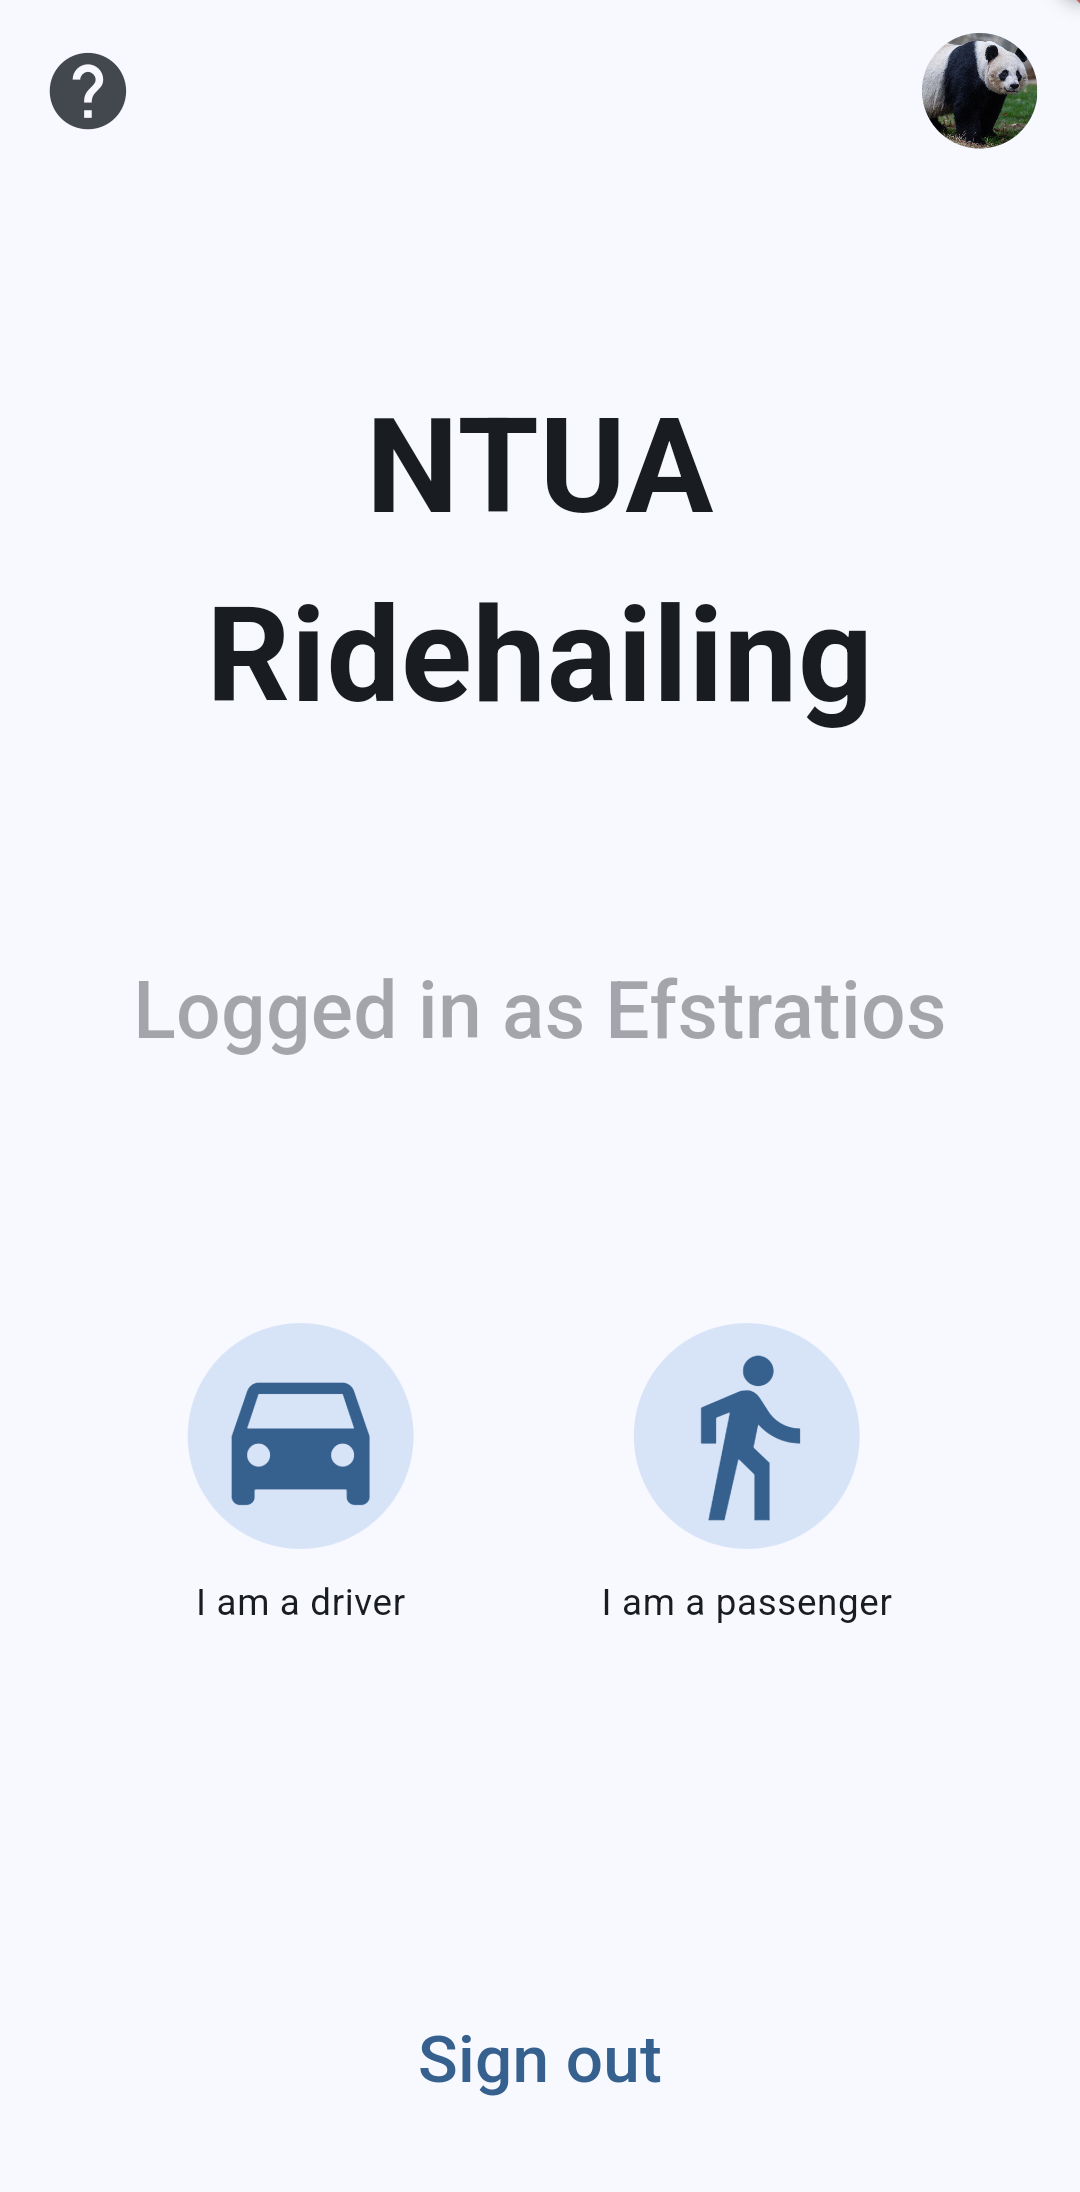
\includegraphics[width=\linewidth,height=0.5\textheight,keepaspectratio]{app_welcome.png}}
    \hfill
    \subcaptionbox{Η οθόνη επιλογής οχήματος του οδηγού.}[0.45\textwidth]{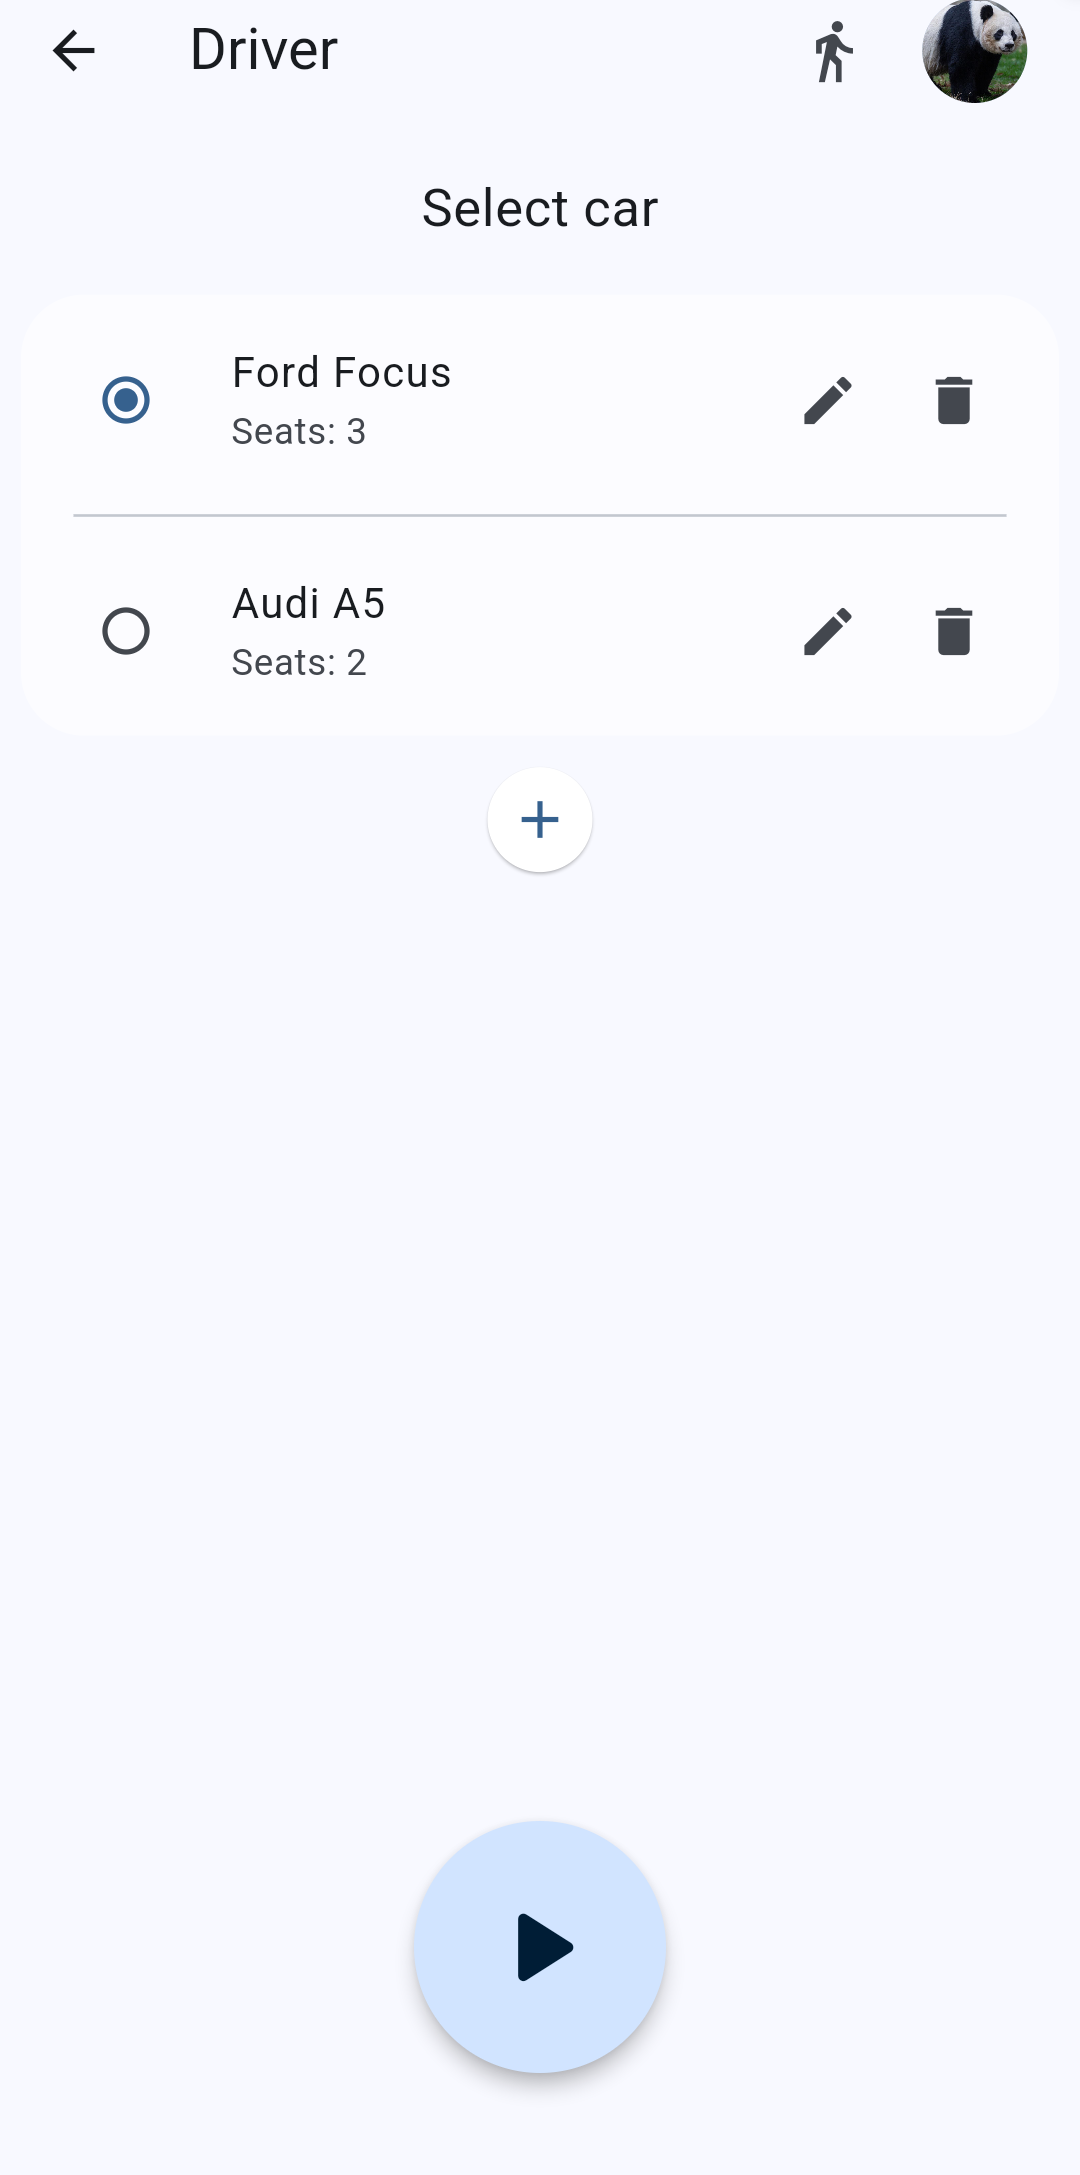
\includegraphics[width=\linewidth,height=0.5\textheight,keepaspectratio]{app_car_list.png}}
    \par\bigskip
    \subcaptionbox{Η οθόνη τροποποίησης ενός οχήματος.}[0.45\textwidth]{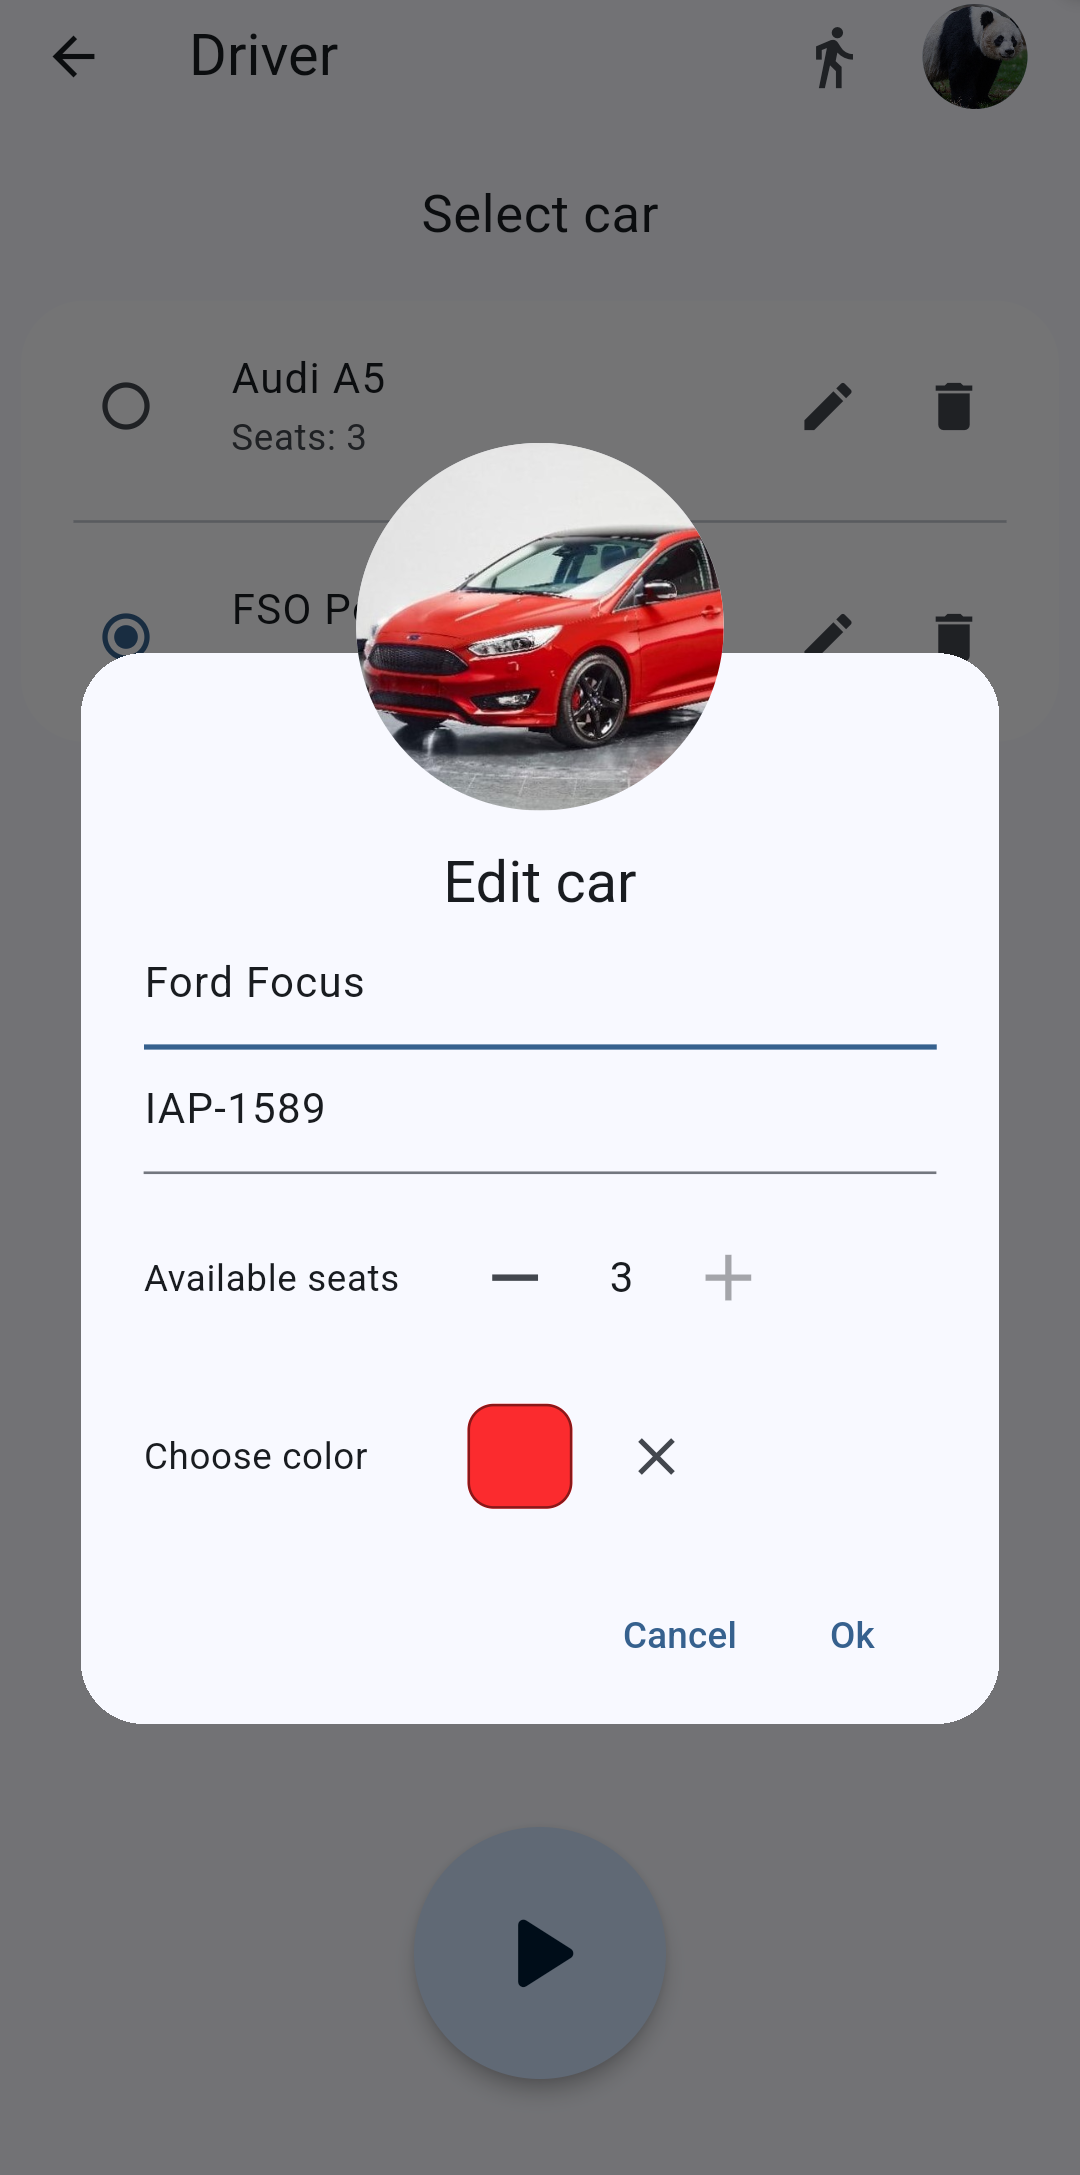
\includegraphics[width=\linewidth,height=0.5\textheight,keepaspectratio]{app_car_edit.png}}
    \hfill
    \subcaptionbox{Η οθόνη όσο ο οδηγός αναμένει την εμφάνιση πεζού.}[0.45\textwidth]{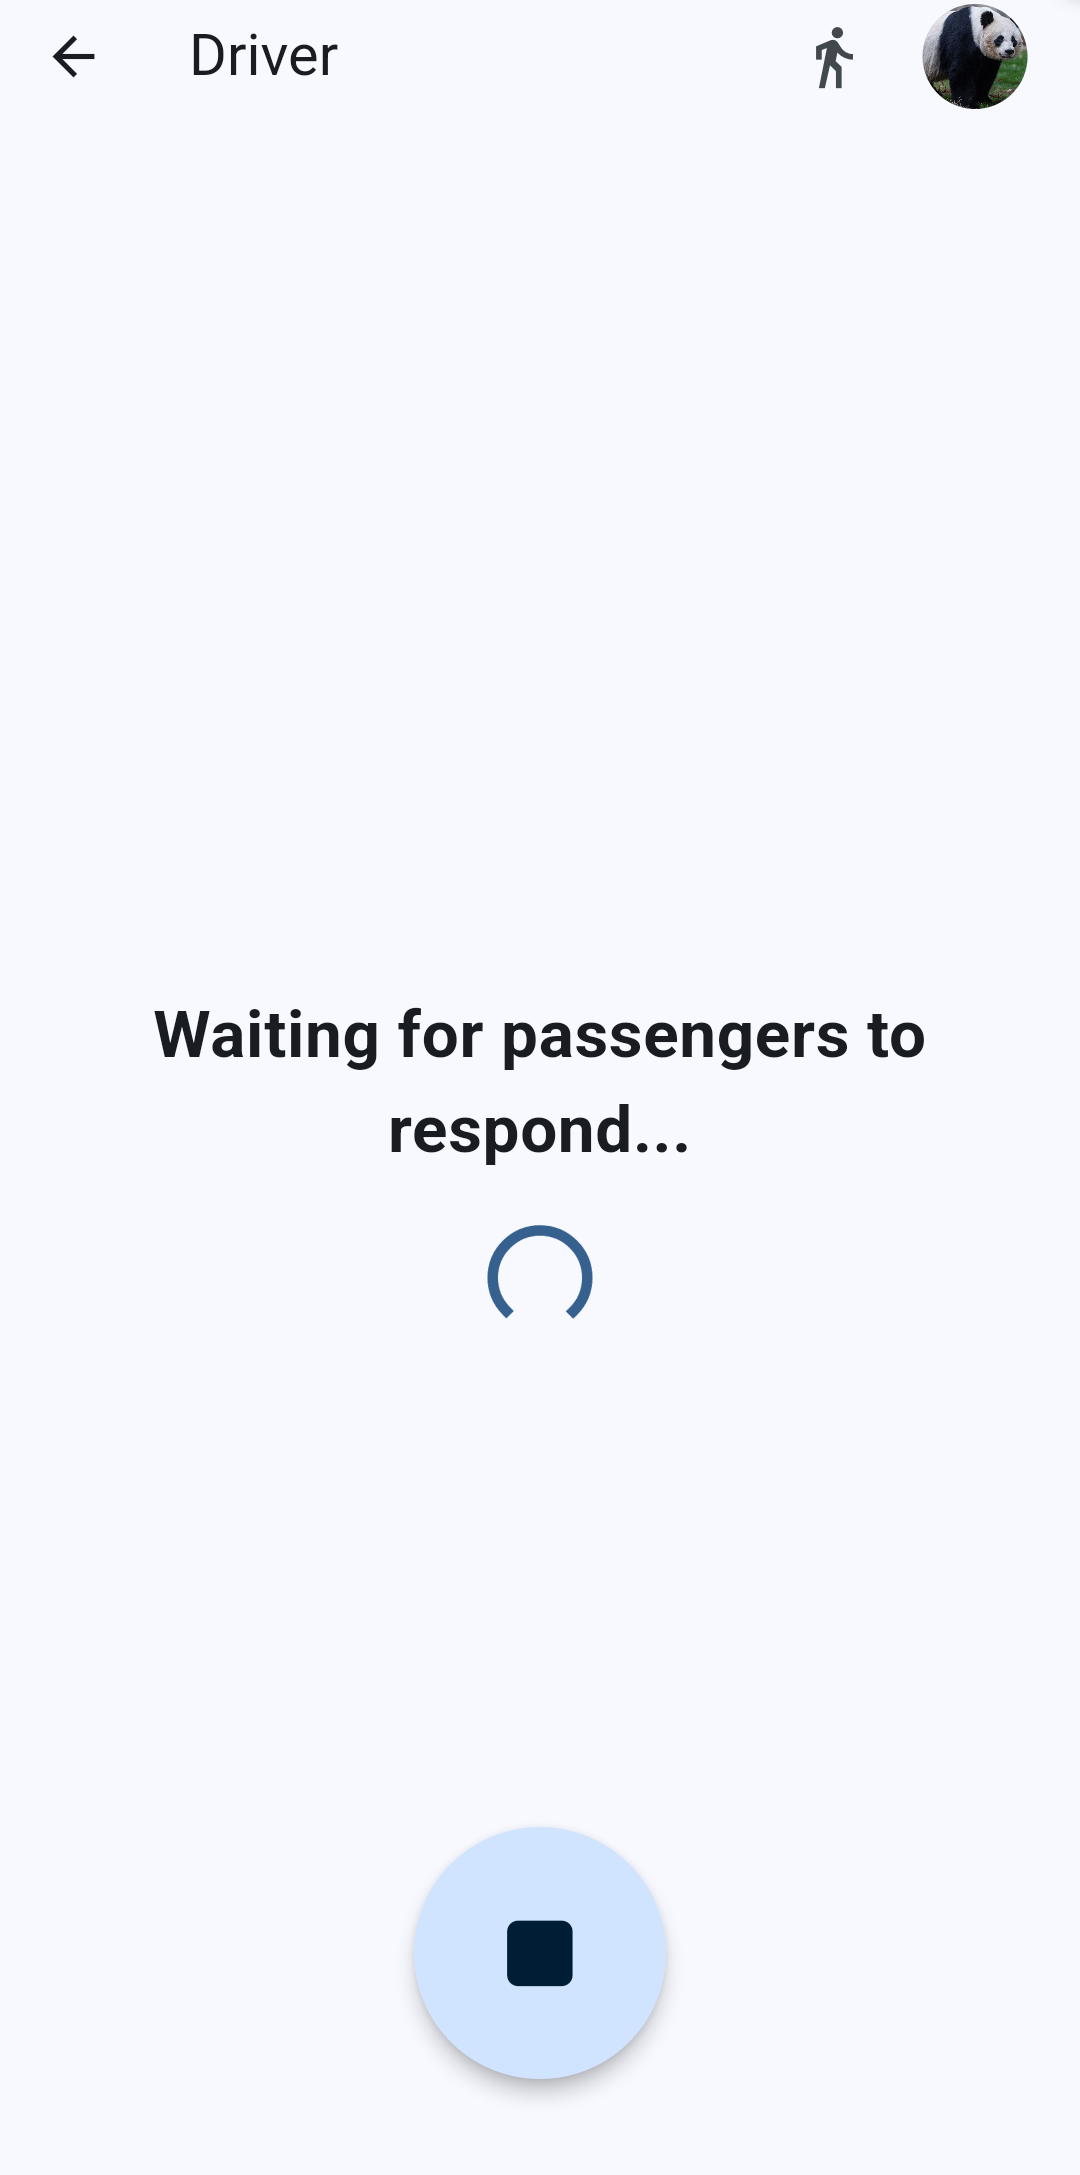
\includegraphics[width=\linewidth,height=0.5\textheight,keepaspectratio]{app_waiting.png}}
\end{figure}

\begin{figure}\ContinuedFloat
    \vspace*{-3cm}
    \subcaptionbox{Η οθόνη του πεζού όταν ερωτάται για την αποδοχή του οδηγού.}[0.45\textwidth]{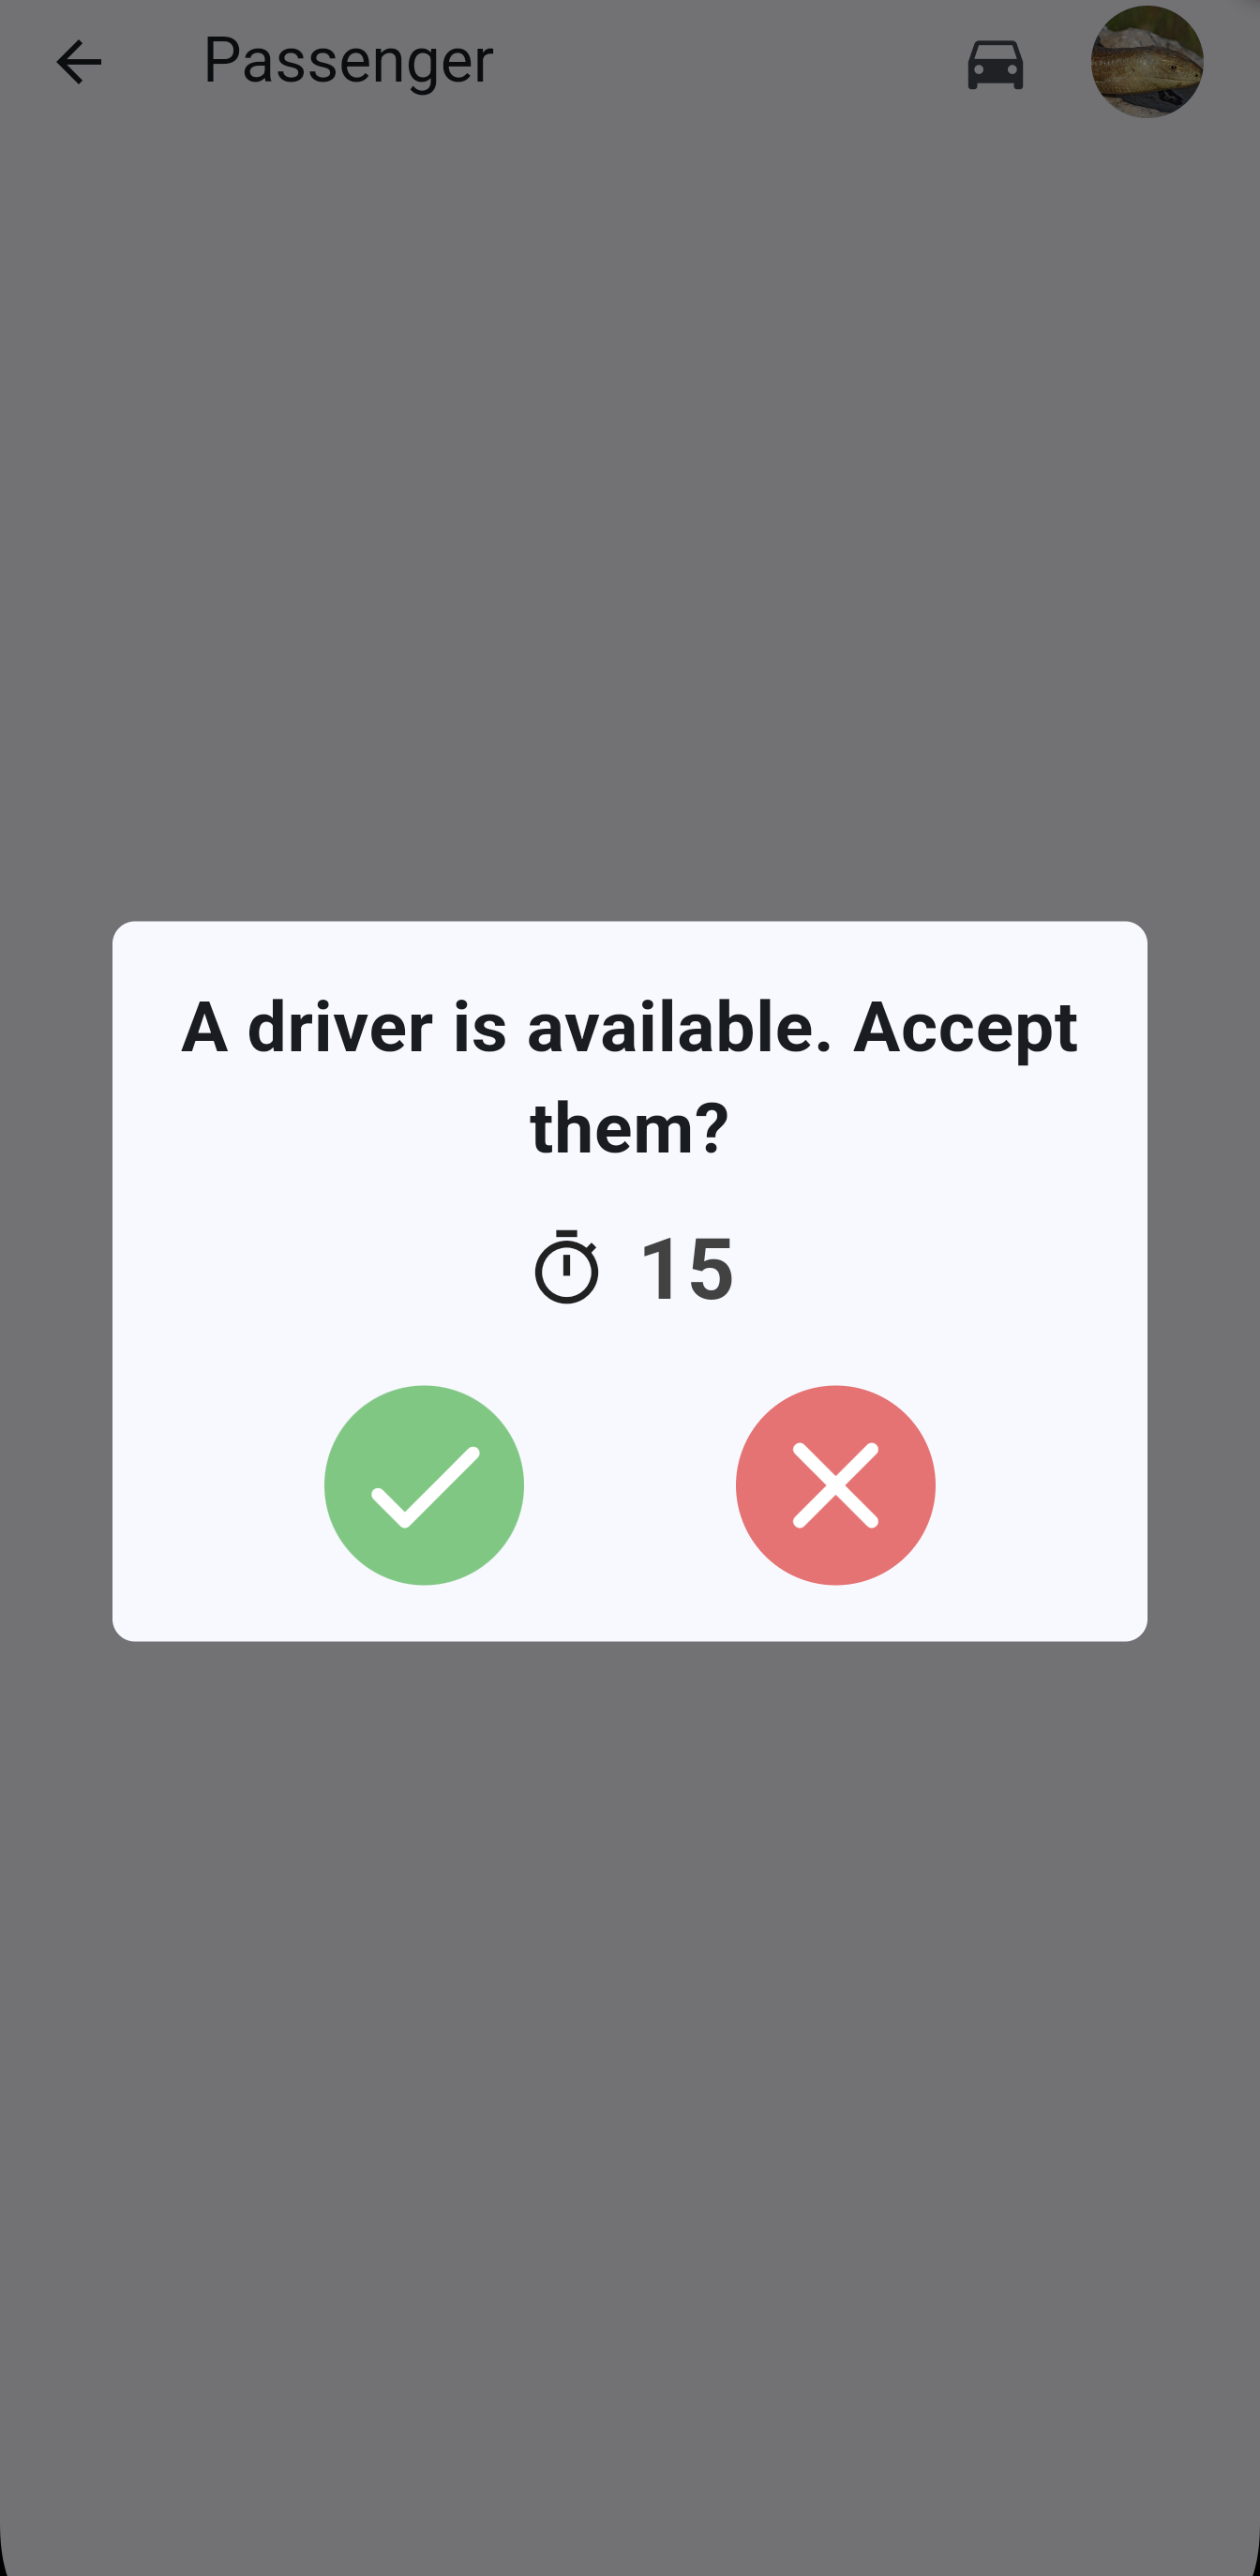
\includegraphics[width=\linewidth,height=0.5\textheight,keepaspectratio]{app_accept.png}}
    \hfill
    \subcaptionbox{Η οθόνη του χάρτη κατά τη διάρκεια της διαδρομής.}[0.45\textwidth]{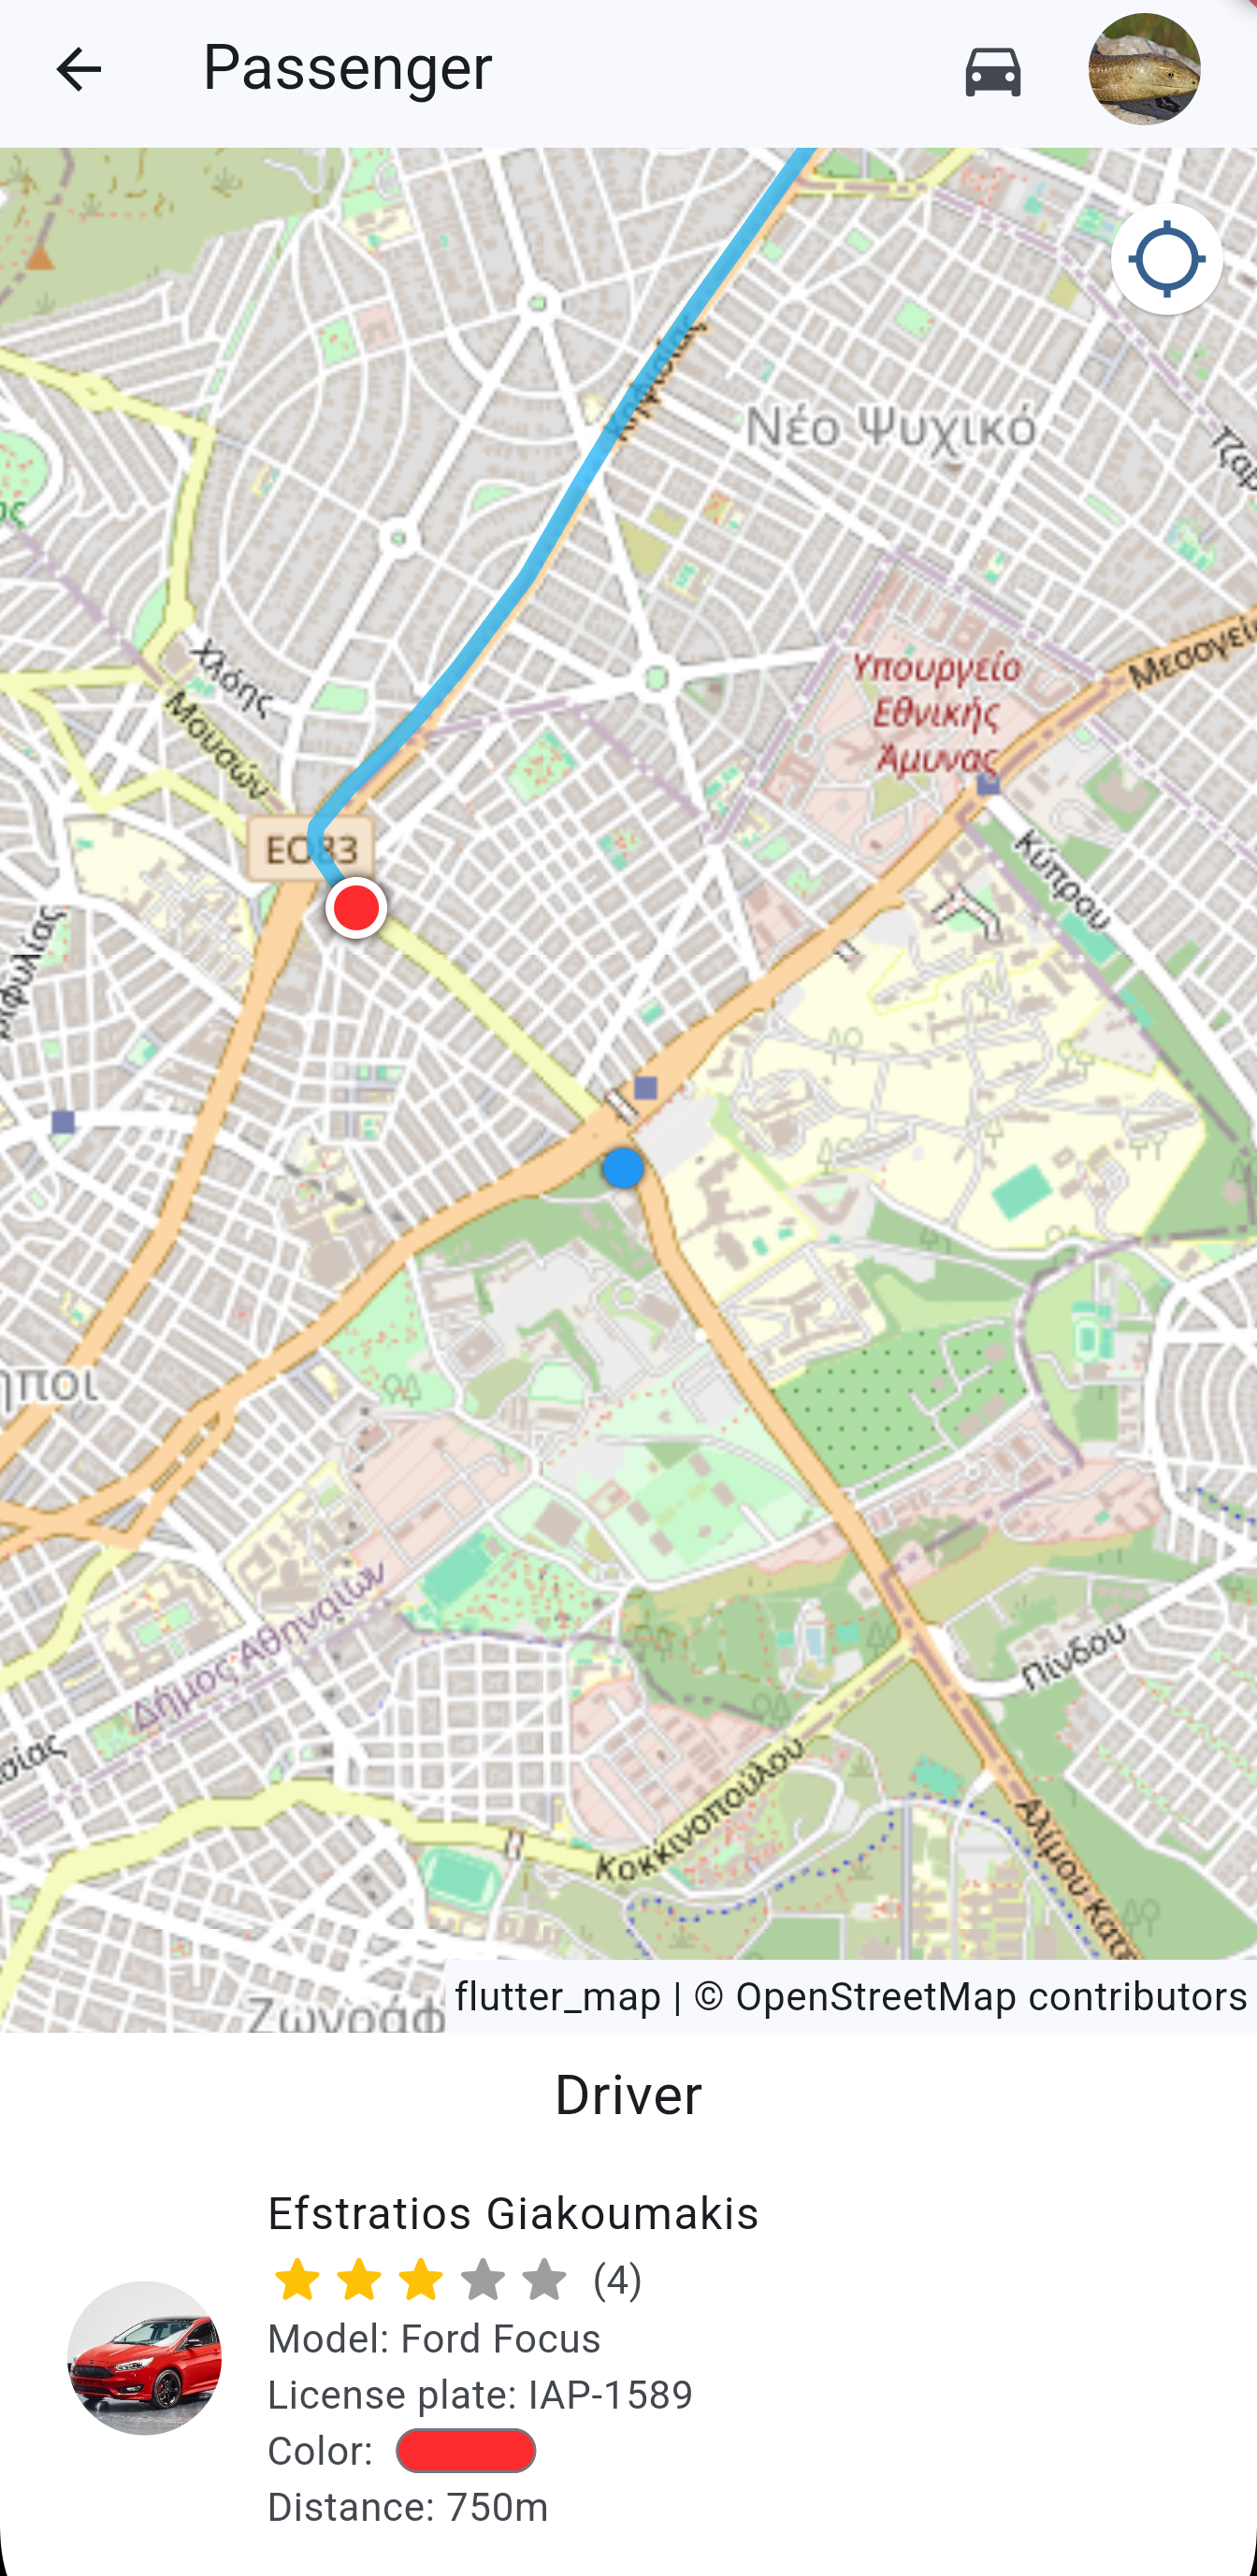
\includegraphics[width=\linewidth,height=0.5\textheight,keepaspectratio]{app_map.png}}
    \par\bigskip
    \subcaptionbox{Η τελική οθόνη αξιόλογησης του οδηγού.}[\textwidth]{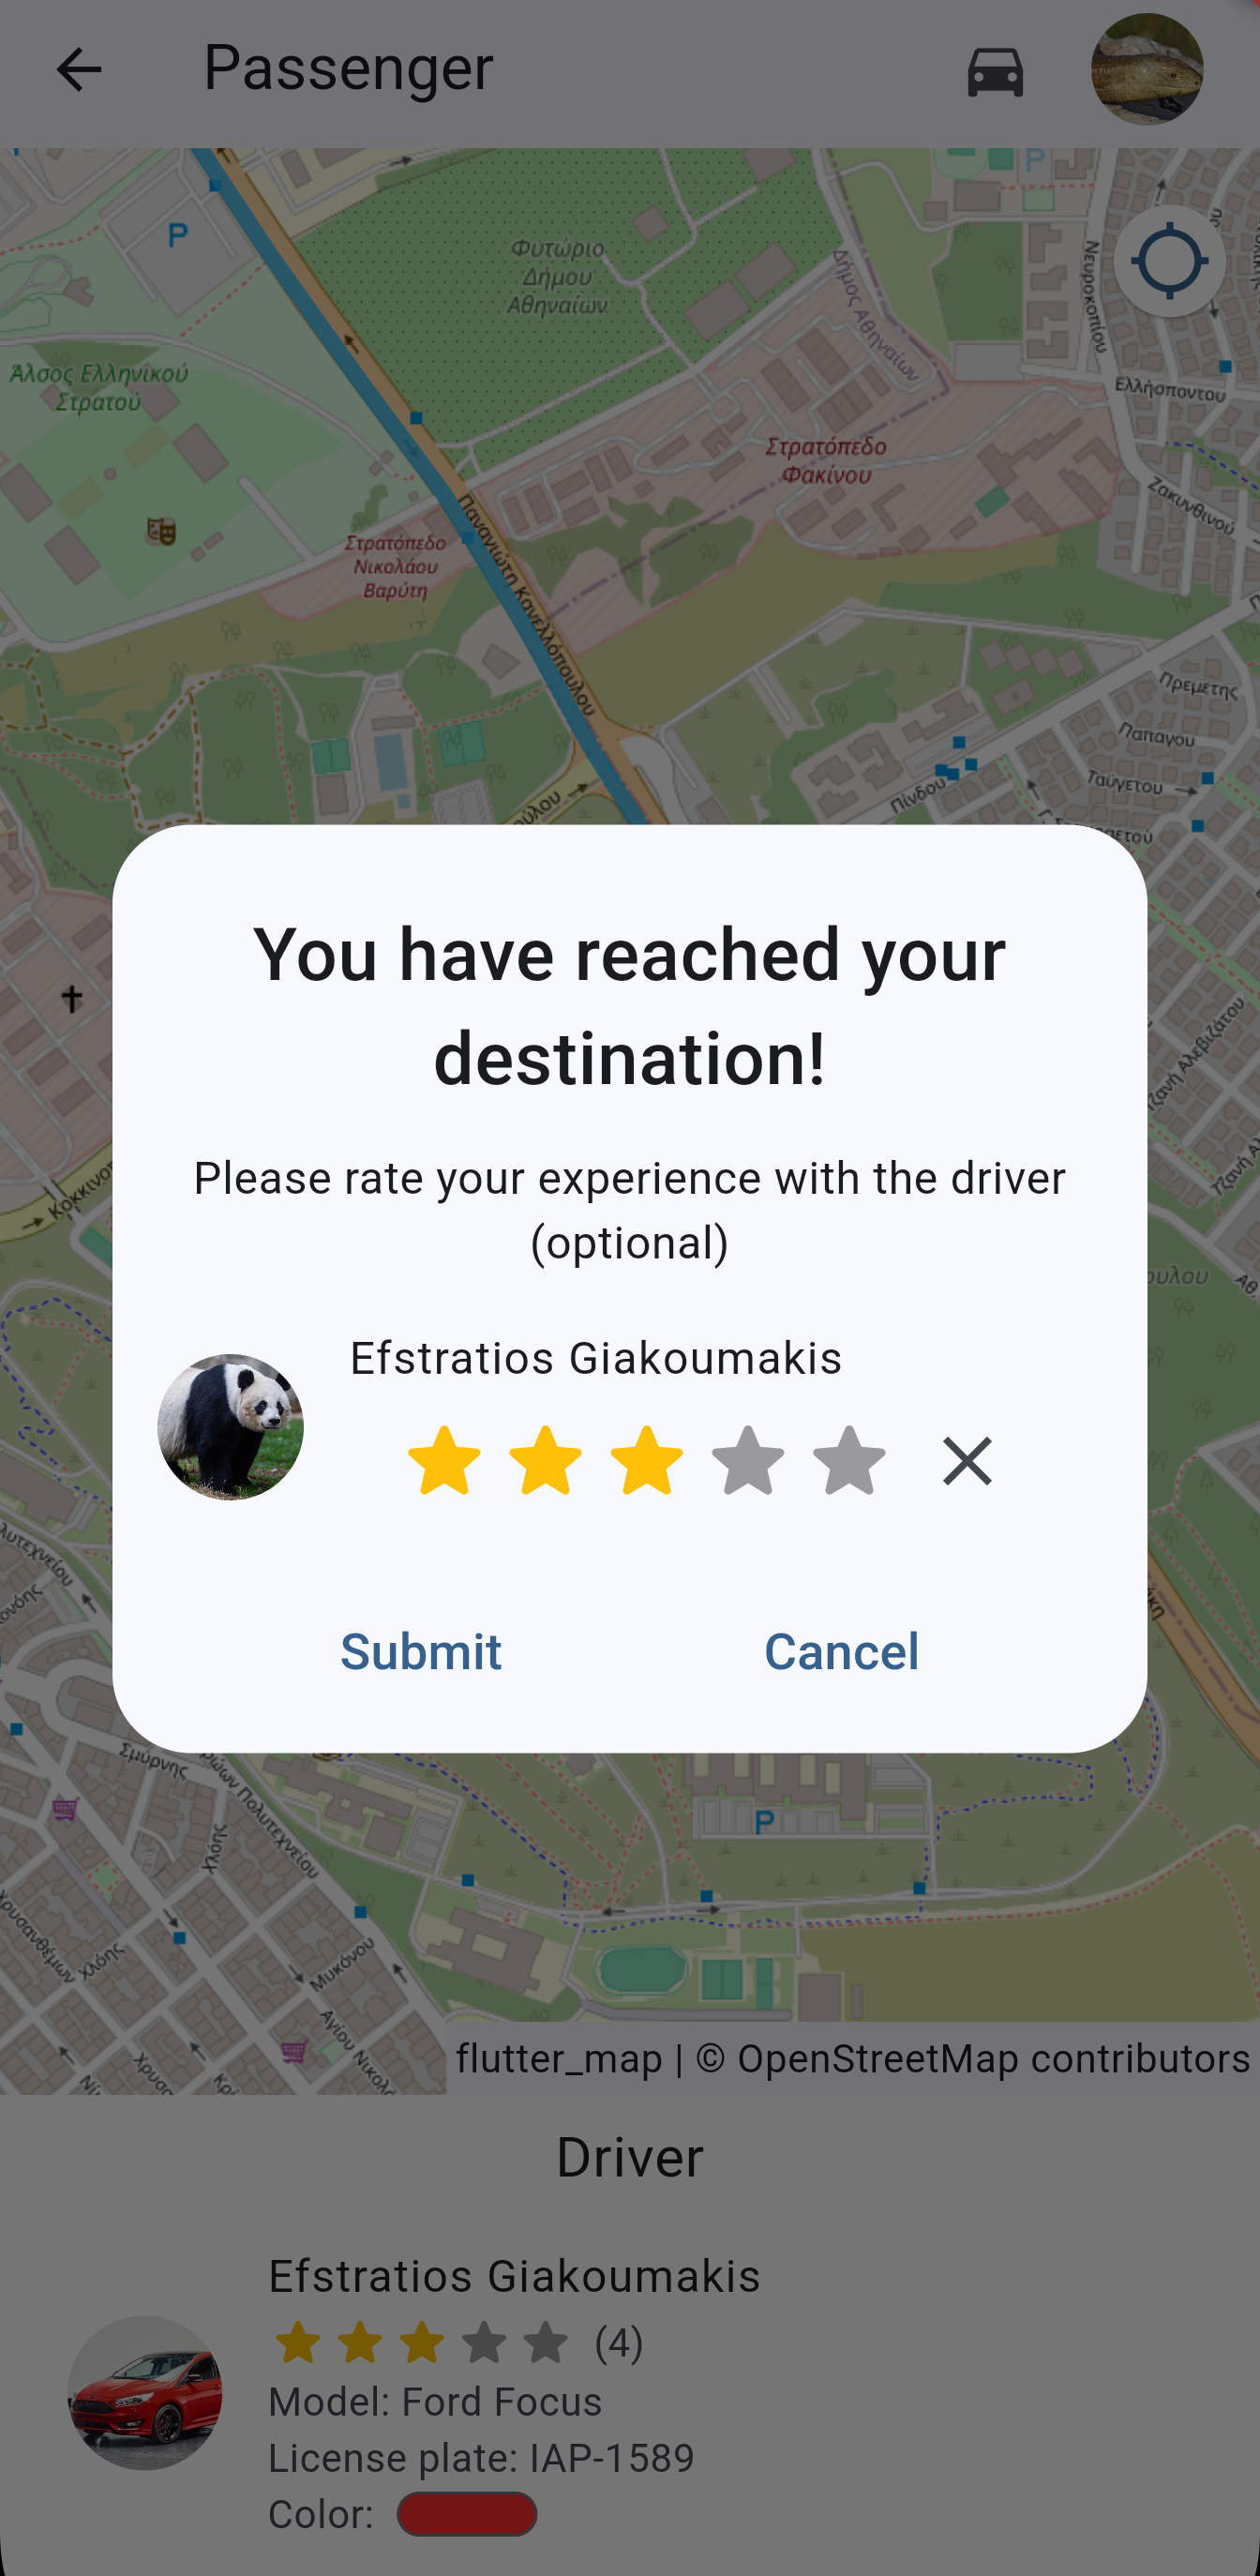
\includegraphics[width=\linewidth,height=0.5\textheight,keepaspectratio]{app_end.png}}
    \caption{Μερικές από τις οθόνες της εφαρμογής}
\end{figure}

\newpage

\section{Παρουσίαση κώδικα}
\subfile{./app_code.tex}

\end{document}